\documentclass[10pt, final]{article}

% Set up page layout
\usepackage[a4paper, margin=1in]{geometry}
% \usepackage{indentfirst}

% Language support
\usepackage{t1enc}
\usepackage[english]{babel}
\usepackage{csquotes}

% Bibliography, refs, citations
\usepackage[sorting=none, backend=biber, style=numeric]{biblatex}
\addbibresource{mmp.bib}
\usepackage{hyperref}
\hypersetup{
	colorlinks=true,
}

% Itemize with letters
\usepackage{enumitem}

% Special math representation (matrix, etc.)
\usepackage{amsmath}
\usepackage{amsfonts}

% Software code
\usepackage{listings}
\lstset{
	language=Python, 
	basicstyle={\color{blue}}
}

% Figures
\usepackage{graphicx}
\usepackage{caption}
\usepackage{subcaption}

% Graphics
\usepackage{tikz}
\usepackage{pgfplots}
\pgfplotsset{compat=1.12}
\usepackage{forest}

% Development tools - only if draft set in the documentclass options
\usepackage{ifdraft}
\ifdraft {\usepackage{showframe}}


\title{Railway Track Fault Detection\\\large Mathemathical Modeling Practice\\}
\author{Tamás DEMUS\\XP4B9D}
\date{Fall Semester 2022}

\begin{document}
	\maketitle
	\tableofcontents
	\section{Introduction}
		Analyzing images and processing the information stored within 
		is a key field of machine learning.
		Classification of different images, identifying and localizing 
		different objects are basic problems.
		Several real-life cases prove the usability of such approach 
		such as traffic sign recognition, object detection or face recognition.
		The target of current research is to endeavour to create an algorithm
		that is able to classify images taken from parts of the rail track
		to classify whether the rail is defect or not.

		In Section \ref{sec:data_desc} the dataset is introduced without any detailed analysis
		to give a first glance where the study is started. 
		Section \ref{sec:prob_stat} the main research questions stated. 
		Following in Section \ref{sec:method} a detailed dexription of the applied methodology
		and toolkits introduced.
		Section \ref{sec:results} presents the results of the study divided according to 
		the main steps of the algorithm.
		In Section \ref{sec:discussion} the results are reflected to the research questions, 
		hopefully leading to positive outcomes.
		Finally Section \ref{sec:conclusion} concludes in the overall achievements.
	\section{Dataset description} \label{sec:data_desc}
		The dataset used for this study is taken from Kaggle webpage \cite*{noauthor_kaggle_nodate}
		and can be downloaded directly from 
		\url{https://www.kaggle.com/datasets/salmaneunus/railway-track-fault-detection}
		\cite*{noauthor_railway_nodate}.
		The dataset is stored in different directories related to their purpose: Train, Validation,
		or Test dataset.
		Inside each directory the classes also splitted to separate directories: Defective or Non defective.
		The directory structure along with the number of images can be seen in Table \ref{table:dir_struct}.
		\begin{table}[!ht]
			\centering
			\begin{tabular}{l c}
				Folder & Number of images \\
				\hline
				./Train/Defective & 150 \\
				./Train/Non defective & 150 \\
				./Validation/Defective & 31 \\
				./Validation/Non defective & 31 \\
				./Test/Defective & 11 \\
				./Test/Non defective & 11 \\
				\hline
			\end{tabular}
			\caption{Dataset directory structure}
			\label{table:dir_struct}
		\end{table}
		The images are taken from different perspectives, either from the top or from the side or from 
		any other direction or angle.
		The photos show different track sections, that could be a close view on the single rail or 
		a full picture taken from the entire rail section.
		The quality of the dataset is spreading between different formats, mostly consisting of jpg files.
		The size of the images are different ranging from very low to very high resolutions.
		The dataset contains only color pictures.
		Some examples are shown in Figure \ref{fig:track_non_def} and Figure \ref{fig:track_def}.
		The total size of the dataset is 2.14 GB.
		\begin{figure}[!ht]
			\centering
			\begin{subfigure}{0.3\textwidth}
				\centering
				\includegraphics[width=\textwidth]{./data/Train/Non defective/7.jpg}
				\caption{Non defective}
			\end{subfigure}
			\begin{subfigure}{0.3\textwidth}
				\centering
				\includegraphics[width=\textwidth]{./data/Train/Non defective/32.jpg}
				\caption{Non defective}
			\end{subfigure}
			\begin{subfigure}{0.3\textwidth}
				\centering
				\includegraphics[width=\textwidth]{./data/Train/Non defective/110.jpg}
				\caption{Non defective}
			\end{subfigure}
			\caption{Example images of non defective track}
			\label{fig:track_non_def}
		\end{figure}
		\begin{figure}[!ht]
			\centering
			\begin{subfigure}{0.3\textwidth}
				\centering
				\includegraphics[width=\textwidth]{./data/Train/Defective/156.jpg}
				\caption{Defective}
			\end{subfigure}
			\begin{subfigure}{0.3\textwidth}
				\centering
				\includegraphics[width=\textwidth]{./data/Train/Defective/182.jpg}
				\caption{Defective}
			\end{subfigure}
			\begin{subfigure}{0.3\textwidth}
				\centering
				\includegraphics[width=\textwidth]{./data/Train/Defective/260.jpg}
				\caption{Defective}
			\end{subfigure}
			\caption{Example images of defective track}
			\label{fig:track_def}
		\end{figure}
	\section{Problem statement} \label{sec:prob_stat}
		The algorithm targets to identify from a picture whether it represents a defective or a non defective 
		track section.
		For this purpose image manipulation technics together with machine learning algorithms, in more detail 
		neural networks applied.
		The problem formulation defines the main questions of the research to be answered:
		\begin{enumerate}[label=Q\arabic*]
			\item \label{itm:Q1} What kind of defects are represented in the images?
			\item \label{itm:Q2} Can these defects detected by applying image manipulation 
				and machine learning approach? 
			\item \label{itm:Q3} What accuracy rate can be achieved with the algorithm?
		\end{enumerate}
	\section{Methodology} \label{sec:method}
		The research can be divided to several major steps, these are described in the subsequent sections.
		The algorithm is developed in Python programming language in a form of a Jupyter notebook.
		In current research the aim was to store the different stages of the processing in different file 
		folders to allow single analytics of each processing step. 
		In each folder the same original structure is retained.
		Therefore the following data folders are differentiated.
		\begin{enumerate}
			\item \lstinline{raw} Contains the raw dataset directly copied from Kaggle.
			\item \lstinline{data} The images after data cleaning in standard format and naming.
			\item \lstinline{augmented} Additional images as result of data augmentation.
			\item \lstinline{preprocessed} The data after image processing, preprocessed for the machine learning
				algorithm. Includes both the original and augmented dataset.
		\end{enumerate}
		\subsection{Data cleaning}
			The images should be brought to the same quality in order to efficiently process them.
			This covers the identification of corrupted files, correct the wrong file formats 
			and the resolution of all issues that prevents the processing of the data along the same pipeline.
			The result of this step should be a data structure that is easy to handle and process further.
			This includes the following information.
			\begin{enumerate}
				\item Type of image, whether it is intended for training, validation or testing.
				\item Indicator of defective or non-defective class, both as integer and as string.
				\item Path of the image directory, filename and their joints as full path.
			\end{enumerate}
		\subsection{Data exploration}
			The target of this step is to get a deep understanding of the pictures contentwise.
			The main properties, such as size, color composition, orientation, what is shown and similar need to be 
			checked with respect to characteristic differences between the distinct classes.
			The size and the mean of the color components is extracted from the images and stored in the dataframe 
			of the images.
			The distribution and correlation of the images color components considering the mean values analyzed.
			A random sample of the images is taken for visualization to study the different defects of the defective class.
			As a final step, the color components were investigated in detail considering the histogram of the component
			values taken for each pixels.
			This is investigated on the RGB color model and the images were converted to HSV model to get a more
			comprehensive view.
		% \subsection{Image processing}
		% \subsection{Data augmentation}
		% \subsection{Neural network configuration}
		% \subsection{Prediction of test data}
		% \subsection{Metrics and evaluation}
	\section{Results} \label{sec:results}
		\subsection{Data cleaning}			
			The raw data from the Kaggle webpage \cite{noauthor_railway_nodate} is copied to the folder \lstinline{raw}.
			This folder is not changed during the data processing, it is used as a starting point and to preserve the 
			original data.
			During data cleaning three different file formats detected, namely \lstinline{webp}, \lstinline{jpeg} 
			and \lstinline{jpg}.
			The filenames show a much wider spread including random names, regular photo labeling (e.g.: DCIM) and others.
			As Tensorflow is not able to work with \lstinline{webp} files and to maintain the same standard along
			the dataset, all files that are not in \lstinline{jpg} format are converted to \lstinline{jpg}.
			During this conversion all the files were renamed applying an integer counter.
			The modified dataset is then stored in the \lstinline{data} folder in the same structure as in the original data.
			
			Second step is to sum all the main information of each image in a single Python DataFrame to allow easy processing.
		\subsection{Data exploration}
			The distribution of the image sizes are shown in Figure \ref{fig:shape_dist}. 
			Please note that higher detail images can be found in the corresponding Jupyter notebook, the aim in this document
			is to explain the evaluation approach and summarize the results.
			Non defective pictures have only 2 shapes, either 3000x4000 or 4000x3000, depending whether it has
			portrait or landscape orientation.
			Defective images have wider distribution in the shapes reaching as high as 8000 pixels and as low as 148 pixels.
			The minimum image size in this case is 148x194 (height x width) and the maximum is 8000x6000.
			All images have 3 color components according to RGB color model.
			\begin{figure}[!ht]
				\centering
				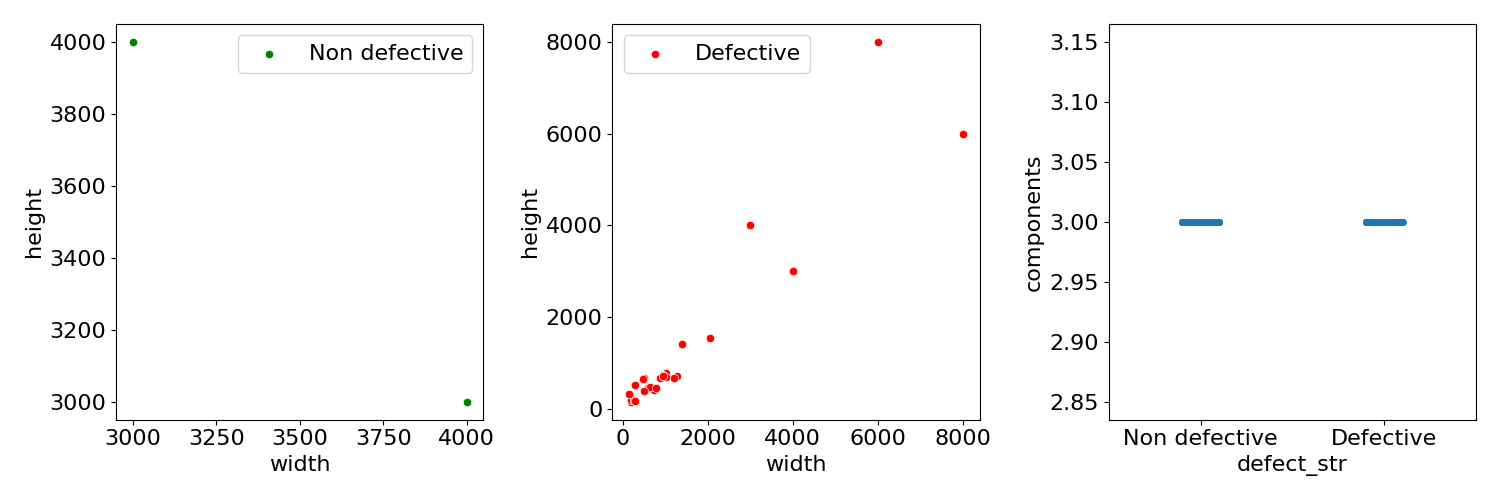
\includegraphics[width=\textwidth]{./plots/shapes.png}
				\caption{Distribution of the image shapes}
				\label{fig:shape_dist}
			\end{figure}

			The distribution and correlation of the mean of the color components with respect to the images is shown on 
			Figure \ref{fig:comp_pair}.
			\begin{figure}[!ht]
				\centering
				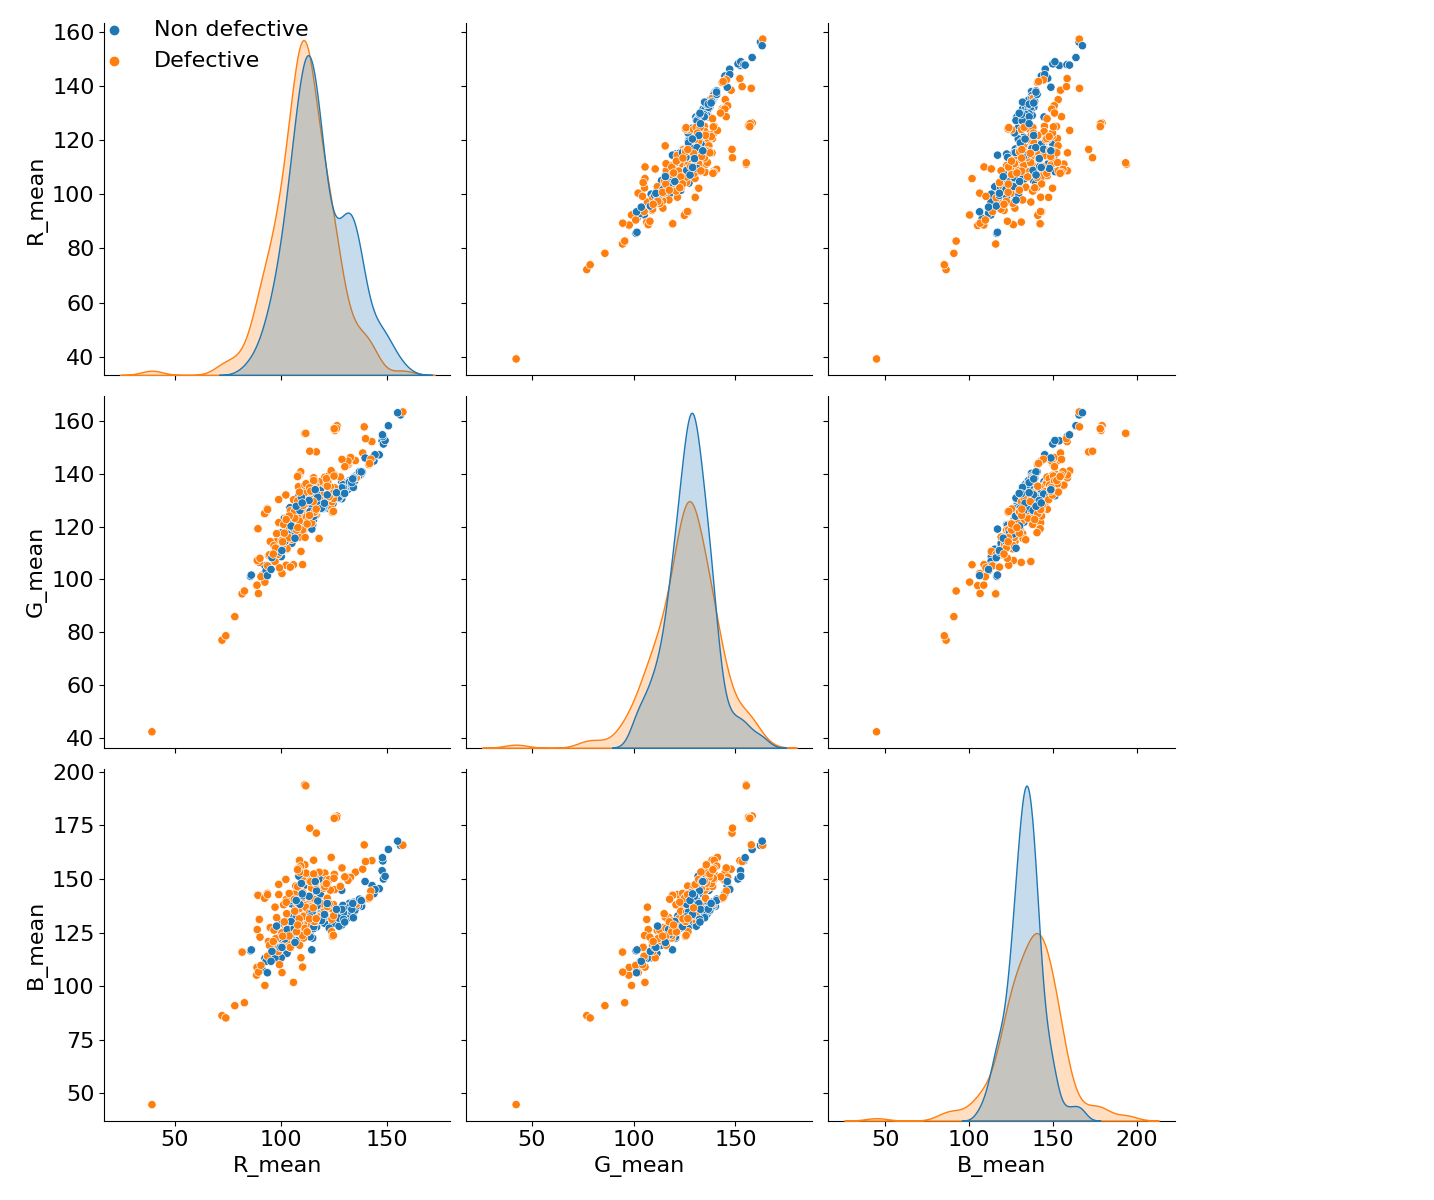
\includegraphics[width=\textwidth]{./plots/comp_pair.png}
				\caption{Color component pair analysis}
				\label{fig:comp_pair}
			\end{figure}
			The different color components show comparable histograms.
			The case of the green and blue component the non defective components show a more narrow distribution.
			The paired color components in both classes represent similar feature spaces.

			During the study of the random samples, the following defects have been identified.
			\begin{enumerate}
				\item Rail cracks. (Figure \ref{fig:def_cracked})
				\item Disjoint rail connections. (Figure \ref{fig:def_disjoint})
				\item Pitting of the rail surface. (Figure \ref{fig:def_pitting})
				\item Improper fixation of the rail. (Figure \ref{fig:def_nofix})
				\item Missing elements, e.g.: screws, springs. (Figure \ref{fig:def_missing})
			\end{enumerate}
			\begin{figure}[!ht]
				\centering
				\begin{subfigure}{0.3\textwidth}
					\centering
					\includegraphics[width=\textwidth]{./data/Train/Defective/287.jpg}
					\caption{Cracked rail}
					\label{fig:def_cracked}
				\end{subfigure}
				\begin{subfigure}{0.3\textwidth}
					\centering
					\includegraphics[width=\textwidth]{./data/Train/Defective/267.jpg}
					\caption{Disjoint rails}
					\label{fig:def_disjoint}
				\end{subfigure}
				\begin{subfigure}{0.3\textwidth}
					\centering
					\includegraphics[width=\textwidth]{./data/Train/Defective/260.jpg}
					\caption{Surface pitting}
					\label{fig:def_pitting}
				\end{subfigure}
				\begin{subfigure}{0.3\textwidth}
					\centering
					\includegraphics[width=\textwidth]{./data/Train/Defective/202.jpg}
					\caption{Wrong fixation}
					\label{fig:def_nofix}
				\end{subfigure}
				\begin{subfigure}{0.3\textwidth}
					\centering
					\includegraphics[width=\textwidth]{./data/Train/Defective/215.jpg}
					\caption{Missing element}
					\label{fig:def_missing}
				\end{subfigure}
				\caption{Identified rail defects}
			\end{figure}
			The magnitude of each defect is varying in a wide range. 
			For example in case of cracked rails, from a crack of a few millimeters up to a missing rail part of several
			centimeters can be found.
			Similarly, surface pitting can range from small cracks on the surface up to severe cases, like shown in
			Figure \ref{fig:def_pitting}.

			The color component analysis on RGB and HSV colormodes revealed no exact differentiation between the classes.
			The component values highly depend on what is represented on the picture and how the photo is taken.
			For example, presence of shadow has a significant impact on the component histogram.
			An example of the analysis is shown on Figure \ref{fig:color_analysis}.
			\begin{figure}[!ht]
				\centering
				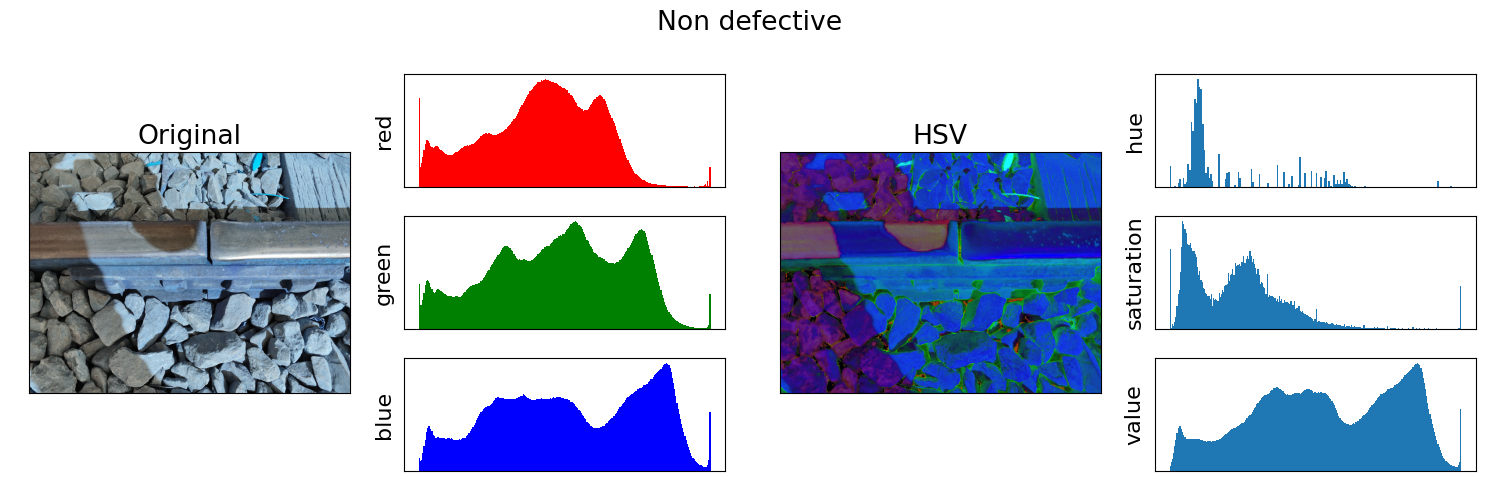
\includegraphics[width=\textwidth]{./plots/comp_analysis_1.png}
				\caption{Color component analysis on RGB and HSV color modes}
				\label{fig:color_analysis}
			\end{figure}
	\section{Discussion} \label{sec:discussion}
	\section{Conclusion} \label{sec:conclusion}
	\listoffigures
	\listoftables
	\printbibliography
\end{document}